\documentclass[main.tex]{subfiles}

\begin{document}

  \section{Superelliptic curves}\label{sec:se_curves}

  \subsection{Definition \& properties}\label{subsec:se_def}

    \begin{defn}\label{def:se_curve}
    In this paper, a superelliptic curve $\cu$ over $\C$ is a smooth projective curve that has an affine model given by an equation of the form
   \begin{equation}\label{eq:aff_model}
    \caff : \quad y^m = f(x) =  c_f \cdot \prod_{k=1}^n (x-x_k),
   \end{equation}
   \end{defn}
   \noindent
   where $m > 1$ and $f \in \C[x]$ is separable of degree $n \ge 3$. Note that we do not assume that $\gcd(m,n) = 1$.

  There are $\delta = \gcd(m,n)$ points $P_{\infty}^{(1)},\dots,P_{\infty}^{(\delta)} \in \cu$ at infinity, that behave differently depending on $m$ and $n$ (see \cite[\S 1]{CT1996} for details).
  In particular, $\infty \in \P^1_{\C}$ is a branch point for $\delta \ne m$. Thus, we introduce the set of finite branch points $X = \X$ as well as the set of all branch points
  \begin{align}\label{eq:branch_points}
         \hat{X} = \begin{cases}   X \cup \{ \infty \} \quad \text{if} \; m  \nmid  d,\\
         X \hfill \text{otherwise.}
     \end{cases}
  \end{align}
  The ramification indices at the branch points are given by $e_x = m$ for all $x \in X$ and $e_{\infty} = \frac{m}{\delta}$. Using the
  Riemann-Hurwitz formula, we obtain the genus of $\cu$ as
  \begin{equation}\label{eq:genus}
    g = \frac{1}{2}( (m-1)(n-1) - \delta + 1).
  \end{equation}
  We denote the corresponding finite ramification points $P_k = (x_k,0) \in \cu$ for $k = 1,\dots,n$.

  \begin{rmk}
   Without loss of generality we may assume $c_f = 1$ (if not, apply the transformation $(x,y) \mapsto (x,\sqrt[m]{c_f}y)$).
  \end{rmk}
  \begin{rmk}
      \label{rmk:moebius}
      For any $\begin{pmatrix}a&b\\c&d\end{pmatrix}\in\PSl(2,\C)$,
      the Moebius transform $\phi:u\mapsto \frac{au+b}{cu+d}$ is an automorphism
      of $\P^1$. By a change of coordinate $x=\phi(u)$ we obtain a different model of $\cu$
      given by the equation
      \begin{equation*}
          \tilde v^m = \tilde f(u)
      \end{equation*}
      where $\tilde f(u)=f(\phi(u))(cu+d)^{\ell m}$ and $v=y(cu+d)^\ell$ for
      the smallest value $\ell$ such that $\ell m\geq n$.

      If the curve was singular at infinity, the singularity is moved to $u=-d/c$ in the new model.
      This happens when $\delta < m$ (so that $\ell m > n$).

  When $\delta=m$ we may apply such a transformation to improve the configuration
  of affine branch points.
  \end{rmk}

  \subsection{Complex roots and branches of the curve}\label{subsec:roots_branches}

  \subsubsection{The complex $m$-th root}

  Working over the complex numbers we encounter several multi-valued functions
  which we will briefly discuss here. Closely related to superelliptic
  curves over $\C$ is the complex $m$-th root.
  Before specifying a branch it is a multi-valued function $y^m = x$
  that defines an $m$-sheeted Riemann surface, whose only branch points
  are at $x = 0,\infty$, and these are totally ramified.

  For $x\in\C$, it is natural and computationally convenient to use the
  \emph{principal branch} of the $m$-th root $\sqrt[m]x$ defined by
  \begin{equation*}
      %\label{eq:principal_mth_root}
      -\frac{π}m<\arg(\sqrt[m]x)\leq\frac{π}m
  \end{equation*}
  which has a branch cut along the negative real axis $]\!-\infty,0]$.
  Crossing it in positive orientation corresponds to multiplication by
  the primitive $m$-th root of unity
  \begin{equation*}
      %\label{eq:zeta}
  \zeta := \zeta_m := e^{\frac{2\pi i }{m}}
  \end{equation*}
  on the surface. In
  particular, the monodromy at $x=0$ is cyclic of order $m$.

  \subsubsection{The Riemann surface}\label{subsec:riemann_surface}

  For an introduction to the theory of Riemann surfaces, algebraic curves and holomorphic covering maps we recommend \cite{Miranda1995}.



   Over $\C$ we can identify the curve $\cu$ with the compact Riemann surface $\cu(\C)$. Since our defining equation
   has the nice form
   $y^m = \prod_{k = 1}^n (x - x_k)$ we view $\cu$ as a Riemann surface with $m$ sheets and
   all computations will be done in the $x$-plane.

   We denote by $\pr : \cu \rightarrow \P^1_{\C}$ the corresponding smooth cyclic branched covering of the projective line
   defined by the $x$-coordinate.

  There
  are $m$ possibilities to continue $y$ as an analytic function following a path in the $x$-plane. This is crucial for the integration
  of differentials on $\cu$. Due to the cyclic structure of $\cu$, they are related in a convenient way:

  We call a \emph{branch of $\cu$} a function $y(x)$ such that
  $y(x)^m = f(x)$ for all $x \in \C$. At every $x$, the branches of $\cu$ only
  differ by a factor $\zeta^l$ for some $l \in \{0,\dots,m-1\}$. Thus, following a path, it is sufficient to know \emph{one} branch that is analytic in a suitable neighborhood. In the
  next paragraph, we will introduce locally analytic branches very explicitly.

  \bigskip

  We obtain an ordering of the sheets relative
  to the analytic branches of $\cu$ by imposing that multiplication by $\zeta$,
  i.e. applying the map $(x,y(x)) \mapsto (x,\zeta y(x))$, corresponds to
  moving one sheet up on the Riemann surface.

   \bigskip


  Consequently, the local monodromy of the cyclic covering $\pr$  is equal and cyclic of order $m$ at every $x_k \in X$
 and the monodromy group is, up to conjugation, the cyclic group $C_m$. This makes it possible to find explicit generators for the
  homology group $\homo$ without specifying a base point, as shown in \S \ref{m-subsec:cycles_homo}.

  \subsubsection{Locally analytic branches}\label{subsubsec:analytic_branches}

  In order to integrate differential forms on $\cu$
  it is sufficient to be able to follow \emph{one} explicit analytic continuation of $y$ along a
  path joining two branch points $a, b \in X$.

  One could of course consider the \emph{principal branch} of the curve
  \begin{equation*}
      y(x) = \sqrt[m]{f(x)},
  \end{equation*}
  but this is not a good model to compute with: it has
  discontinuities along the curves $f^{-1}(]-\infty,0]$, all
  wandering around the $x$-plane in an unpredictable way (see Figure \ref{fig:mth_root_principal}).
  These are the branch cuts of $y(x)$, crossing them in positive direction
  requires multiplying by $\zeta$ in order to follow an analytic continuation.

  %, and one must multiply by $\zeta$
  %to crossing them in positive direction
  %corresponds to moving one sheet up on the Riemann surface. With
  %Similar to the complex $m$-th root, we can assume that crossing the branch
  %cut at $x_k \in X$ in positive direction corresponds to multiplication by
  %$\zeta$ on the Riemann surface.

  A better option is to split the product as follows:
  assume that $(a,b) = (-1,1)$. Then the function
  \begin{equation*}
      y(x) = \prod_{x_k\in X}\sqrt[m]{x-x_k}
  \end{equation*}
  has $n$ branch cuts parallel to the real line (see Figure \ref{fig:mth_root_product}).
  However, one of them lies exactly on the interval $[-1,1]$ we are interested in. We work around this
  by taking the branch cut towards $+\infty$ for each branch point $x_k$ with positive real part, writing
  \begin{equation*}
      y(x) = e^{\frac{iπr^+}m}\prod_{\Re(x_k)\leq0}\sqrt[m]{x-x_k} \prod_{\Re(x_k)>0}\sqrt[m]{x_k-x},
  \end{equation*}
  where $r^+$ is the number of points with positive real part.

  \begin{figure}[H]
      \begin{center}
          \subfloat[principal branch]{
          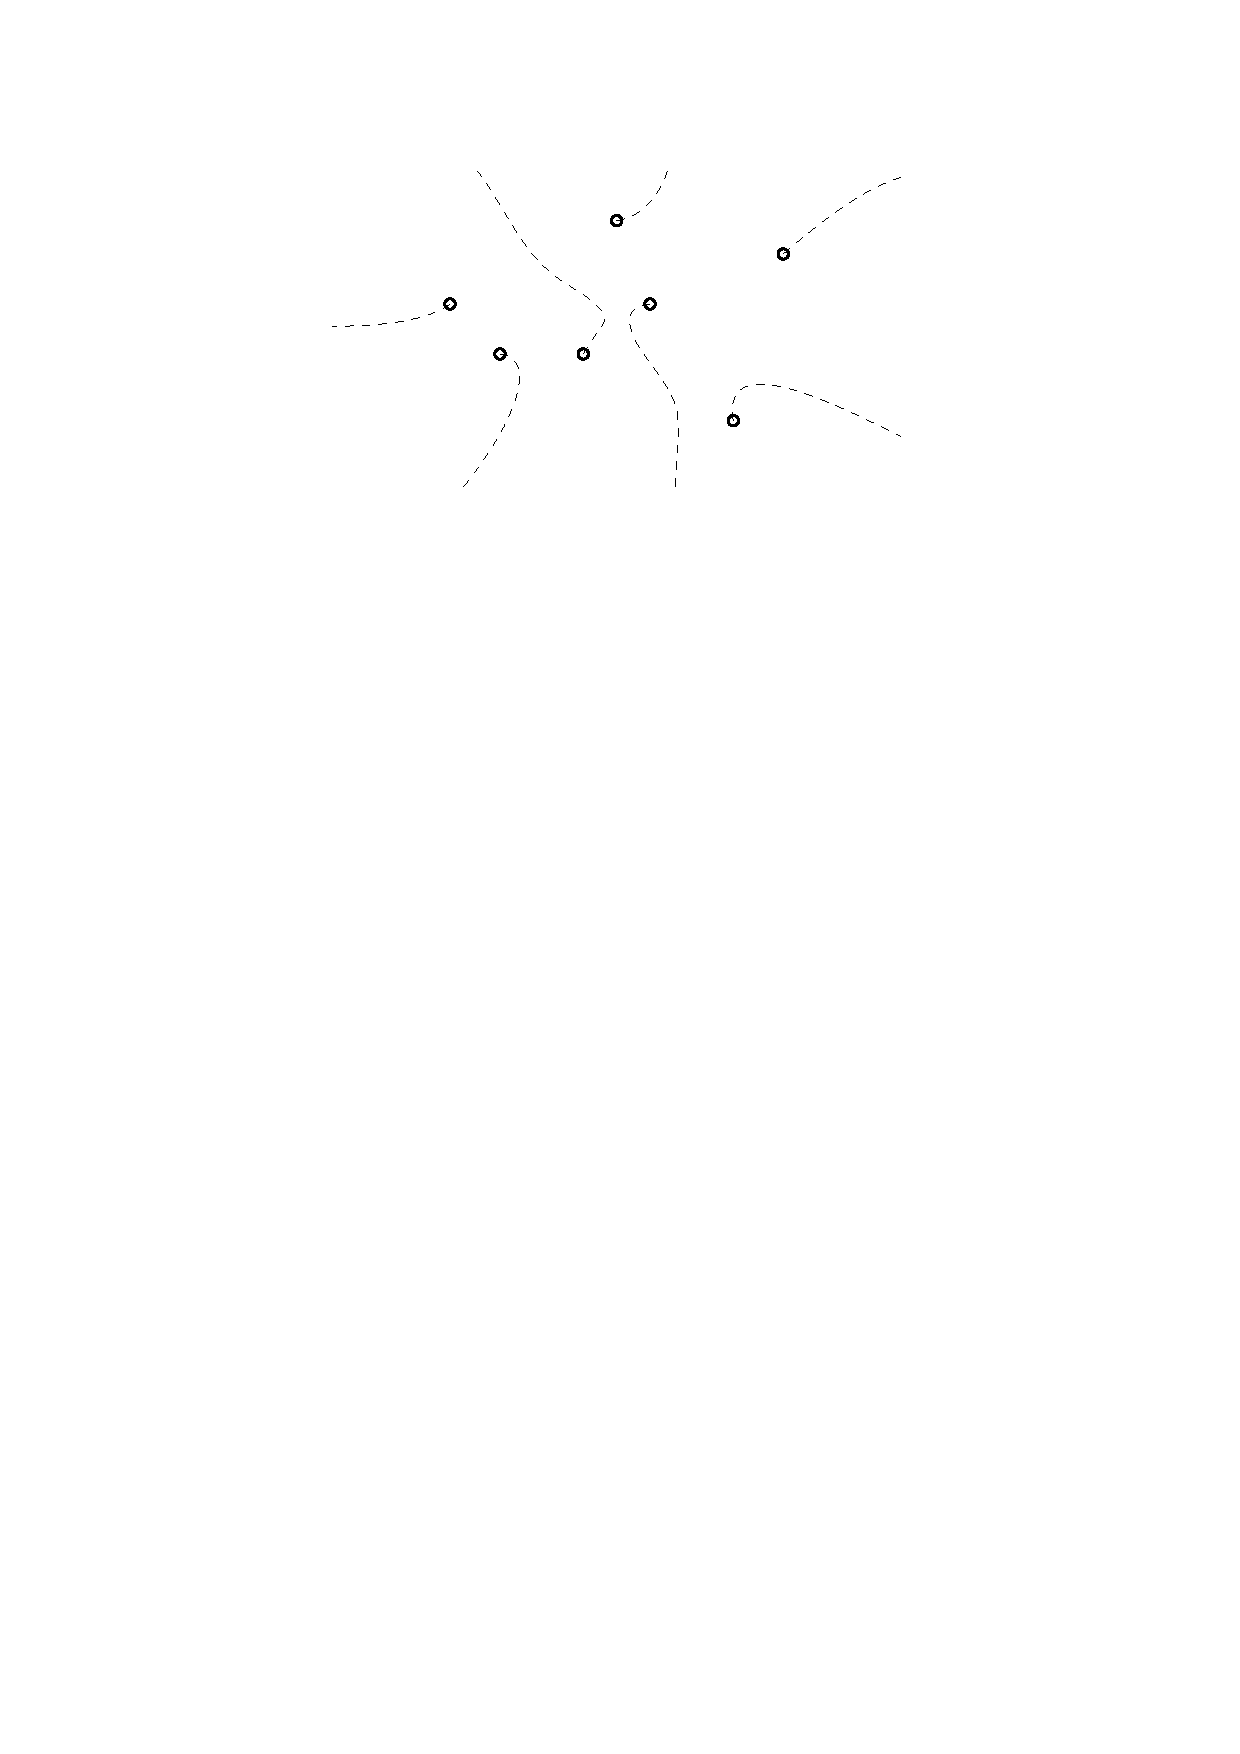
\includegraphics[width=.3\linewidth,page=1]{images/branch_cuts.pdf}
          \label{fig:mth_root_principal} }
          \subfloat[product]{ \includegraphics[width=.3\linewidth,page=2]{images/branch_cuts.pdf}\label{fig:mth_root_product} }
          \subfloat[$\yab$]{ \includegraphics[width=.3\linewidth,page=3]{images/branch_cuts.pdf}\label{fig:mth_root_signed} }
      \end{center}
      \caption{Branch cuts of different $m$-th roots.}
  \label{fig:mth_root_pol} \end{figure}

  In general we proceed in the same way: For branch points $a,b \in X$ we consider the affine linear
  transformation
  \begin{equation*}
      \label{def:xab}
      \xab : u \mapsto \frac{b-a}{2}\left(u+\frac{b+a}{b-a}\right),
  \end{equation*}
  which maps $[-1,1]$ to the complex line segment $[a,b]$, and denote the inverse map by
  \begin{equation*}
      \label{def:uab}
      \uab : x \mapsto \frac{2x-a-b}{b-a}.
  \end{equation*}


   We split the image of the branch points under $\uab$ into the following subsets
  \begin{equation}\label{eq:uab_image}
      \set{ \uab(x), x\in X} = \set{-1,1} \cup U^+ \cup U^-,
  \end{equation}
  where points in $U^+$ (resp. $U^-$) have strictly positive (resp. non-positive) real part.

  Then the product
  \begin{equation}
      \label{eq:ytab}
      \ytab(u) = \prod_{u_k\in U^-} \sqrt[m]{u-u_k}\prod_{u_k\in U^+}\sqrt[m]{u_k-u}
  \end{equation}
  is holomorphic on a neighborhood $ε_{a,b}$ of $[-1,1]$ which we can take as
  an ellipse \footnote{we will exhibit such a neighborhood in Section \ref{m-subsec:gauss_chebychev_integration}}
  containing no point $u_k\in U^-\cup U^+$, while the term corresponding to $a,b$
  \begin{equation*}
      \sqrt[m]{1-u^2}
  \end{equation*}
  has two branch cuts $]-\infty,-1]$ and $[1,\infty[$, and is holomorphic on the complement
  $\overline U$ of these cuts.

  We can now define a branch of the curve
  \begin{equation}
      \label{eq:def_yab}
      \yab(x) =   C_{a,b} \yt_{a,b}( \uab(x) ) \sqrt[m]{1 - \uab(x)^2}
  \end{equation}
  by setting $r = 1+\#U^+ \bmod 2$ and choosing the constant
  \begin{equation}
      C_{a,b} = \left(\frac{b-a}{2}\right)^{\frac{n}{m}} e^{\frac{\pi i}{m}r}
  \end{equation}
  such that $\yab(x)^m = f(x)$.

  The function $\yab(x)$ has $n$ branch cuts all parallel to $[a,b]$ in outward direction and
  is holomorphic inside $]a,b[$ (see Figure \ref{fig:mth_root_signed}).

  More precisely, $\vab = \xab(ε_{a,b}\cap \overline U)$,
  is an ellipse-shaped neighborhood of $]a,b[$ with two segments removed
  (see Figure \ref{m-fig:set_vab})
  on which the local branch $\yab$ is well defined and holomorphic.

  \begin{figure}[H] \begin{center} 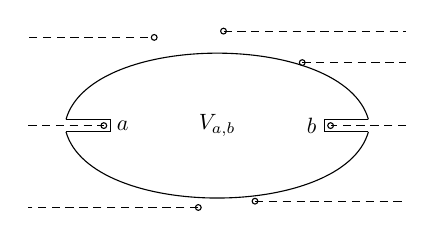
\begin{tikzpicture}[scale=0.8, every node/.style={scale=0.8}]
  \draw (-1.5,0) node {$a$};  \draw (1.5,0) node {$b$}; \draw (0,0) node {$V_{a,b}$};
  \draw (-1.8,0) circle (1.3pt); \draw (1.8,0) circle (1.3pt);
    \draw [densely dashed] (-3,0) -- (-1.8,0);   \draw [densely dashed] (3,0) -- (1.8,0);
    \draw (-2.4,0.1) .. controls (-2,1.5) and (2,1.5) .. (2.4,0.1);
    \draw (-2.4,-0.1) .. controls (-2,-1.5) and (2,-1.5) .. (2.4,-0.1);
    \draw (-2.4,-0.1) -- (-1.7,-0.1); \draw (2.4,-0.1) -- (1.7,-0.1);
    \draw (-2.4,0.1) -- (-1.7,0.1); \draw (2.4,0.1) -- (1.7,0.1);
    \draw (-1.7,0.1) -- (-1.7,-0.1); \draw (1.7,0.1) -- (1.7,-0.1);
    % Other branch points
    \draw (-1,1.4) circle (1.3pt);
    \draw [densely dashed] (-1.1,1.4) -- (-3,1.4);
    \draw (-0.3,-1.3) circle (1.3pt);
    \draw [densely dashed] (-0.3,-1.3) -- (-3,-1.3);
    \draw (1.35,1) circle (1.3pt);
    \draw [densely dashed] (1.35,1) -- (3,1);
    \draw (0.6,-1.2) circle (1.3pt);
    \draw [densely dashed] (0.6,-1.2) -- (3,-1.2);
     \draw (0.1,1.5) circle (1.3pt);
    \draw [densely dashed] (0.1,1.5) -- (3,1.5);
\end{tikzpicture}


  \end{center} \caption{Holomorphic neighborhood of $\yab$.}
  \label{fig:set_vab} \end{figure}



We sum up the properties of these local branches:

 \begin{prop}\label{prop:yab}
      Let $a,b\in X$ be branch points such that $X\cap\,]a,b[\,=\varnothing$.
      Then, with the notation as above, the functions
      $\ytab$ \eqref{eq:ytab} and $\yab$ \eqref{eq:def_yab}
      satisfy
     \begin{itemize}
         \item $\ytab$ is holomorphic and does not vanish on $ε_{a,b}$,
         \item $\yab(x) = C_{a,b} \ytab(\uab(x)) \sqrt[m]{1-\uab(x)^2}$ is holomorphic
         on $\vab$,
         \item $\yab(x)^m = f(x)$ for all $x\in\C$,
         \item $\yab(x),\zeta\yab(x),\dots,\zeta^{m-1}\yab(x)$ are the $m$ different analytic continuations of $y$ on $\vab$.
     \end{itemize}
     Moreover, we can assume that for $x \in \vab$, applying the map $(x,\yab(x)) \mapsto (x,\zeta^l\yab(x))$ corresponds to moving up $l \in \Z/m\Z$ sheets on the Riemann surface.
 \end{prop}

 \subsection{Cycles and homology}\label{subsec:cycles_homo}

   For us, a \emph{cycle} on $\cu$ is a smooth oriented closed path in $\pi_1(\cu)$.
   For simplicity we identify all cycles with their homology classes in $\homo = \pi_1(\cu)/[\pi_1(\cu),\pi_1(\cu)]$.

   In the following we present an
   explicit generating set of $\homo$ that relies on the locally analytic branches $\yab$ as defined in \eqref{m-eq:def_yab} and the superelliptic structure of $\cu$.

   Let $a, b \in X$ be branch points such that $X\cap]a,b[=\varnothing$, where  $[a,b]$ is the oriented line segment connecting $a$ and $b$.

   By Proposition \ref{m-prop:yab} the lifts of $[a,b]$ to $\cu$ are given by
   \begin{equation*}\label{eq:def_path_ab}
      \gamma^{(l)}_{[a,b]} = \{  (x,\zeta^l \yab(x))  \mid  x \in [a,b]  \}, \quad l \in \Z/m\Z.
   \end{equation*}
   Similarly, we obtain lifts of $[b,a]$ by reversing the orientation of $\gamma^{(l)}_{[a,b]}$. We denote
   \begin{equation*}\label{eq:def_path_ba}
      -\gamma^{(l)}_{[a,b]} = \{  (x,\zeta^l \yab(x))  \mid  x \in [b,a]  \}, \quad l \in \Z/m\Z.
   \end{equation*}
   These are smooth oriented paths that connect $P_a = (a,0)$ and $P_b = (b,0)$ on $\cu$. We obtain cycles by concatenating these lifts in the following way:
    \begin{equation}\label{eq:def_cyabl}
      \cyabl = \gamma^{(l)}_{[a,b]} \cup -\gamma^{(l+1)}_{[a,b]} \in \pi_1(\cu).
   \end{equation}
   \begin{defn}[Elementary cycles]\label{def:elem_cycles}
       We say $\cyab = \cyab^{(0)}$ is an \emph{elementary cycle} and call $\cyabl$ its \emph{shifts} for $l \in \Z/m\Z$.
   \end{defn}
   In $\pi_1(\cu)$
   shifts of elementary cycles are homotopic to cycles that encircle $a$ in negative and $b$ in positive orientation, once each and do not encircle any other branch point. 
   This is possible because we can always find
   an open neighborhood $V$ of $[a,b]$ such that $V \cap X = \{a,b\}$ and thus the homotopy class of a cycle is not changed by deformations within $V$.
   By definition of $\yab$ the branch cuts at the end points are outward and parallel to $[a,b]$. Thus, we have the following useful visualizations of $\cyabl$ on $\cu$:
   \begin{figure}[H]
      \begin{center}
   % Tikz File 'tikz_pic_13.tex'
\begin{tikzpicture}
     \draw (-1.8,2) node {$a$};  \draw (1.8,2) node {$b$};
     \draw [densely dashed] (-3.0,3) -- (-1.8,3);  \draw [densely dashed] (1.8,3) -- (3.0,3); \draw (-1.8,3) circle (1.3pt); \draw (1.8,3) circle (1.3pt);
      \draw (-1.8,3) -- (1.8,3) [halfarrow2];
   \draw [densely dashed] (-3.0,1) -- (-1.8,1);  \draw [densely dashed] (1.8,1) -- (3.0,1); \draw (-1.8,1) circle (1.3pt); \draw (1.8,1) circle (1.3pt);
\draw (-1.8,1) -- (1.8,1) [halfarrow1];
      
      
      \draw (3.5,2) node {$\sim$};
      
           \draw (5.2,2) node {$a$};  \draw (8.8,2) node {$b$};
     \draw [densely dashed] (4.0,3) -- (5.2,3);  \draw [densely dashed] (8.8,3) -- (10,3); \draw (5.2,3) circle (1.3pt); \draw (8.8,3) circle (1.3pt);
     
\draw (4.5,3) .. controls (4.5,2.4) and (6,2.6) .. (7,3) [halfarrow2];
\draw (7,3) .. controls (8,3.4) and (9.5,3.6) .. (9.5,3) [halfarrow2];

   \draw [densely dashed] (4,1) -- (5.2,1);  \draw [densely dashed] (8.8,1) -- (10,1); \draw (5.2,1) circle (1.3pt); \draw (8.8,1) circle (1.3pt);
\draw (4.5,1) .. controls (4.5,1.6) and (6,1.4) .. (7,1) [halfarrow1];
\draw (7,1) .. controls (8,0.6) and (9.5,0.4) .. (9.5,1) [halfarrow1];
\end{tikzpicture}

      \end{center}
    \caption{Homotopic representations of a cycle $\cyabl$.}
    \label{fig:elem_cycle}
\end{figure}

  \bigskip

  As it turns out, we do not need all elementary cycles and their shifts to
  generate $\homo$, but only those that correspond to edges in a \emph{spanning tree},
  that is a subset $E\in X\times X$ of directed edges $(a,b)$ such that all branch points
  are connected without producing any cycle. It must contain exactly $n-1$ edges.
  The actual tree will be chosen in \S \ref{subsec:spanning_tree} in order to minimize
  the complexity of numerical integration.

    \medskip
  For an edge $e = (a,b) \in E$, we denote by $\gamma_e^{(l)}$ the shifts of
  the corresponding elementary cycle $\cyab$.

  \begin{thm}\label{thm:gen_set}
      Let $E$ be a spanning tree for the branch points $X$.
   The set of cycles $\Gamma = \left\{  \gamma_{e}^{(l)}  \mid  0 \le l <m-1,  e \in E  \right\}$ generates $\homo$.
  \end{thm}
  \begin{proof}
  Denote by $\alpha_a \in \pi_1(\P^1 \setminus \hat{X})$ a closed path that encircles the branch point $a \in \hat{X}$ exactly once. Then,  due to the relation $1 = \prod_{a \in \hat{X}} \alpha_a$,
  $\pi_1(\P^1 \setminus \hat{X})$ is freely generated by $\{ \alpha_a \}_{a \in X}$, i.e. in the case $\delta \ne m$ we can omit $\alpha_{\infty}$. \abstand
  Since our covering is cyclic, we have that $
  \pi_1(\cu \setminus \pr^{-1}(\hat{X})) \isom \ker(\pi_1(\P^1 \setminus \hat{X}) \overset{\Phi}{\To} \Aut(\cu \setminus \pr^{-1}(\hat{X})))$ where $\Aut(\cu \setminus \pr^{-1}(\hat{X})) \isom C_m
  \subset S_m$
  and $\Phi(\alpha_a)$ is cyclic of order $m$ for all $a \in X$. Hence, for every word $\alpha = \alpha_1^{s_1}\dots \alpha_n^{s_n} \in \pi_1(\P^1 \setminus \hat{X})$ we have that
  $\alpha \in \ker(\Phi) \eq \sum_{i=1}^n s_i \equiv 0 \bmod m$. \abstand
  We now claim that $\pi_1(\cu \setminus \pr^{-1}(\hat{X})) = \langle  \alpha_a^{-s} \alpha_b^{s},  \alpha_a^m   \mid  s \in \Z, a,b \in X  \rangle$
  and prove this by induction on $n$: for $\alpha = \alpha_1^{s_1}$, $m$ divides $s_1$ and therefore $\alpha$ is generated by $\alpha_1^m$. For $n > 1$ we write
  $\alpha = \alpha_1^{s_1}\dots \alpha_n^{s_n} = (\alpha_1^{s_1} \dots \alpha_{n-1}^{s_{n-1}+s_n})(\alpha_{n-1}^{-s_n}\alpha_n^{s_n})$. \abstand
  We obtain the fundamental group of $\cu$ as
  $\pi_1(\cu) \isom \pi_1(\cu \setminus \pr^{-1}(\hat{X})) / \langle  \alpha_a^{e_a}  \mid  a \in \hat{X}  \rangle$, which is generated by
  $\{  \alpha_a^{-s} \alpha_b^{s}  \mid  s \in \Z/m\Z,  a,b \in X  \}$. %$(*)$ 
  \abstand
  All branch points $a,b \in X$ are connected by a path $(a,v_1,\dots,v_t,b)$ in the spanning tree, so we can write $\alpha_a^{-s} \alpha_b^{s} = (\alpha_a^{-s}\alpha_{v_1}^{s})
  (\alpha_{v_1}^{-s}\alpha_{v_2}^{s})\dots(\alpha_{v_{t-1}}^{-s}\alpha_{v_t}^{s})(\alpha_{v_t}^{-s}\alpha_b^{s})$ and hence we have that
  $\{ \alpha_a^{-s} \alpha_b^{s}  \mid  s \in \Z/m\Z,  (a,b) \in E \}$ generates $\pi_1(\cu)$ and therefore $\homo$. \abstand
%     All that is left to see, is that for each edge $e = (a,b) \in E$ there exists a bijection $\varphi_e$ between
%   $\{  \gamma_e^{(l)}  \mid  l \in \Z/m\Z  \} \overset{\varphi_e}{\longleftrightarrow} \{  \alpha_a^{-s} \alpha_b^{s}  \mid  s \in \Z/m\Z  \}$: \abstand
  If we choose basepoints $p_0 \in \P^1 \setminus \hat{X}$ for $\pi_1(\P^1 \setminus \hat{X})$ and $P_0 \in \pr^{-1}(p_0)$ for $\pi_1(\cu \setminus \pr^{-1}(\hat{X}))$ and $\pi_1(\cu)$ respectively, then,
  depending on the choice of $P_0$, for all $e = (a,b) \in E$ there exists $l_0 \in \Z/m\Z$ such that $\gamma_e^{(l_0)}$ is homotopic to $\alpha_a^{-1} \alpha_b$ in $\pi_1(\cu,P_0)$.
   In $\homo$ we have that $\alpha_a^{-s}\alpha_b^{s} = ( \alpha_a^{-1}\alpha_b)^s$, so we obtain the other powers by concatenating
  the shifts $\prod_{l = 0}^{s-1} \gamma_e^{(l_0+l)} = (\alpha_a^{-1}\alpha_b)^s$.
  This implies $1 = \prod_{l = 0}^{m-1} \gamma_e^{(l_0+l)} = \prod_{l = 0}^{m-1} \gamma_e^{(l)}$ and
   $$\{  \alpha_a^{-s} \alpha_b^{s}  \mid  s \in \Z/m\Z  \} \subset  \langle  \gamma_e^{(l)}
  \mid  0 \le l < m-1 \rangle,$$ and therefore $\homo = \langle  \Gamma  \rangle$.
  \end{proof}

  \begin{rmk}
  \begin{itemize}
   \item[$\bullet$] For $\delta = 1$, we have that $\# \Gamma = (m-1)(n-1) = 2g$. Therefore, $\Gamma$ is a basis for $\homo$ in that case.
   \item[$\bullet$] In the case $\delta = m$, the point at infinity is not a branch point. Leaving out one finite branch point in the spanning tree results in only $n-2$ edges. Hence, we easily find a subset
   $\Gamma' \subset \Gamma$ such that
   $\# \Gamma' = (m-1)(n-2) = 2g$ and $\Gamma'$ is a basis for $\homo$.
%    \item[$\bullet$] In step $(*)$ of the proof, filling in the points above infinity creates relations among
%   these generators:
%   $1 = (\prod_{a \in X} \alpha_a)^{k \cdot e_{\infty}}$, $k = 1,\dots,\delta$. This corresponds to the term $-\delta+1$ in the formula \eqref{m-eq:genus} for the genus of $\cu$.
  \end{itemize}
  \end{rmk}

\subsection{Differential forms}\label{subsec:diff_forms}

    The computation of the period matrix and the Abel-Jacobi map requires a basis of $\hd$ as a $\C$-vector space. In this section we provide a basis that only
   depends on $m$ and $n$ and is suitable for numerical integration. \abstand
    Among the meromorphic differentials
    \begin{align*}
 \WM = \left\{  \omega_{i,j}   \right\}_{\substack{1 \le i \le n-1, \\ 1 \le j \le m-1}} \quad \text{with} \quad \omega_{i,j} = \frac{x^{i-1}\dx}{y^j},
  \end{align*}
  there are exactly $g$ that are holomorphic  and they can be found by imposing a simple combinatorial condition on $i$ and $j$.
 The following proposition is basically a more general version of
  \cite[Proposition 2]{CT1996}.

   \bigskip

     \begin{prop}\label{prop:holom_diff}
 Let $\delta = \gcd(m,n)$. The following differentials form  a $\C$-basis of $\hd$:
 \begin{equation*}\label{eq:holm_diff}
   \W =  \left\{  \omega_{i,j} \in \WM  \mid  -mi + jn - \delta \ge 0  \right\}
 \end{equation*}
     \end{prop}
     \begin{proof}
      First we show that the differentials in $\W$ are holomorphic.
      Let $\w_{i,j} = x^{i-1}y^{-j} \dx \in \WM$. We write down the relevant divisors
      \begin{align*}
       \div(x) & = \sum_{k=1}^m \left(0,\zeta^k\sqrt[m]{f(0)}\right) - \frac{m}{\delta} \cdot \sum_{l = 1}^{\delta} P_{\infty}^{(l)}, \\
       \div(y) & = \sum_{k = 1}^n P_k - \frac{n}{\delta} \cdot \sum_{l = 1}^{\delta}  P_{\infty}^{(l)}, \\
       \div(\dx) & = (m-1)\sum_{k = 1}^n P_k - \left(\frac{m}{\delta} + 1\right)\cdot \sum_{l = 1}^{\delta}  P_{\infty}^{(l)}.
      \end{align*}
     Putting together the information, for $P \in \cu$ lying over $x_0 \in \P^1_{\C}$, we obtain
     \begin{align}\label{eq:diff_cases}
      v_P(\omega_{i,j}) & = (i-1) v_P(x) + v_P(\dx)  - j v_P(y) = 
 \begin{cases}
  \ge 0 \hfill \text{if} \; x_0 \ne x_k,\infty, \\
  m-1-j \ge 0 \quad \text{if} \; x_0 = x_k, \\
  \frac{(-mi-\delta+jn)}{\delta} \hfill \text{if}\;  x_0 = \infty.
 \end{cases}
     \end{align}
     We conclude: $\omega_{i,j} \in \WM$ is holomorphic if and only if $\omega_{i,j} \in \W$. \abstand
     Since the differentials in $\W$ are clearly $\C$-linearly independent, it remains to show that
     there are enough of them, i.e. $\#\W = g$.
     \medskip

     Counting the elements in $\W$ corresponds to counting lattice points
     $(i,j) \in \Z^2$ in the trapezoid given by the faces
     \begin{align*}
 1 \le i \le n-1,\\
 1 \le j \le m-1, \\
 i \le \frac{n}{m}j - \frac{\delta}{m}.
     \end{align*}
      \begin{figure}[H]
      \begin{center}
   \begin{tikzpicture}
\draw (-0.7,0) -- (8,0) [->]; \draw (8.5,0) node {$j$};
\draw (0,-0.7) -- (0,4) [->]; \draw (0,4.5) node {$i$};
\draw (1,-0.05) -- (1,0.05); \draw (1,-0.4) node {$1$};
\draw (2,-0.05) -- (2,0.05); \draw (2,-0.4) node {$2$};
\draw (3,-0.05) -- (3,0.05); \draw (3,-0.4) node {$3$};
\draw (4,-0.05) -- (4,0.05); \draw (4,-0.4) node {$4$};
\draw (5,-0.05) -- (5,0.05); \draw (5,-0.4) node {$5$};
\draw (6,-0.05) -- (6,0.05); \draw (6,-0.4) node {$6$};
\draw (7,-0.05) -- (7,0.05); \draw (7,-0.4) node {$7$};
\draw (-0.05,1) -- (0.05,1); \draw (-0.4,1) node {$1$};
\draw (-0.05,2) -- (0.05,2); \draw (-0.4,2) node {$2$};
\draw (-0.05,3) -- (0.05,3); \draw (-0.4,3) node {$3$};
\draw[gray] (1,1) -- (1,3);
\draw[gray] (1,1) -- (7,1);
\draw[gray] (7,1) -- (7,3);
\draw[gray] (1,3) -- (7,3);
\draw[gray] (0,-0.5) -- (8,3.5);
\filldraw [gray] (1,1) circle (1pt);
\filldraw [gray] (1,2) circle (1pt);
\filldraw [gray] (1,3) circle (1pt);
\filldraw [gray] (2,1) circle (1pt);
\filldraw [gray] (2,2) circle (1pt);
\filldraw [gray] (2,3) circle (1pt);
\filldraw (3,1) circle (1pt);
\filldraw [gray] (3,2) circle (1pt);
\filldraw [gray] (3,3) circle (1pt);
\filldraw (4,1) circle (1pt);
\filldraw [gray] (4,2) circle (1pt);
\filldraw [gray] (4,3) circle (1pt);
\filldraw (5,1) circle (1pt);
\filldraw (5,2) circle (1pt);
\filldraw [gray] (5,3) circle (1pt);
\filldraw (6,1) circle (1pt);
\filldraw (6,2) circle (1pt);
\filldraw [gray] (6,3) circle (1pt);
\filldraw (7,1) circle (1pt);
\filldraw (7,2) circle (1pt);
\filldraw (7,3) circle (1pt);
\end{tikzpicture}
      \end{center}
    \caption{The points below the line correspond to holomorphic differentials.
    Illustrated is the case $n=4,m=8$, and thus $g = 9$.}
    \label{fig:holom_diff}
\end{figure}

Summing over the vertical lines of the trapezoid, we find the following formula that counts the points.
     \begin{align}\label{eq:r_j}
 \#\W & = \sum_{j = 1}^{m-1} \floor*{\frac{n}{m}j - \frac{\delta}{m}} = \sum_{j = 1}^{m-1} \frac{nj-\delta-r_j}{m} =
  \frac{n}{m} \sum_{j=1}^{m-1} j - \frac{m-1}{m}\delta - \frac{1}{m} \sum_{j=1}^{m-1} r_j,
     \end{align}
      where $r_j = nj - \delta  \bmod m$.

The desired equality  $\#\W = \frac{1}{2}((n-1)(m-1)-\delta+1) = g$ immediately follows from
\begin{lemma}
      \begin{equation*}\label{eq:r_j2}
       \sum_{j=1}^{m-1} r_j = \frac{1}{2}(m^2 - (\delta+2)m + 2\delta).
      \end{equation*}
\end{lemma}
\begin{proof}\let\qed\relax
      Let $l := \frac{m}{\delta}$. First we note that $r_j = r_{j+l}$:
      $$r_{j+l} = n(j+l) - \delta  \bmod m = nj + \frac{n}{\delta}m - \delta  \bmod m =  nj - \delta  \bmod m =  r_j,$$
      and hence
      \begin{align}\label{eq:r_j3}
       \sum_{j=1}^{m-1} r_j = \delta \cdot \sum_{j=1}^{l} r_j - r_m = \delta \cdot \sum_{j=1}^{l} r_j - (-\delta + m).
      \end{align}
      Furthermore, $r_j$ can be written as a multiple of $\delta$:
      $$r_j = \delta \left(\frac{n}{\delta}j - 1\right)  \bmod m.$$
      From $\gcd(\frac{n}{\delta},l) = 1$ we conclude $\left\{  \frac{n}{\delta}j - 1  \bmod l  \mid  1 \le j \le l  \right\} = \{  0,\dots,l-1  \}$.
      Therefore,
      \begin{align}\label{eq:r_j4}
       \sum_{j = 1}^l r_j = \sum_{j = 0}^{l-1} \delta j = \delta \cdot \frac{l(l-1)}{2},
      \end{align}
      and thus \eqref{m-eq:r_j3} and \eqref{m-eq:r_j4} imply
      $$\sum_{j=1}^{m-1} r_j = \delta \cdot \sum_{j=1}^{l} r_j + \delta - m = \delta^2 \cdot \frac{l(l-1)}{2} + \delta - m = \frac{1}{2}(m^2 - (\delta+2)m + 2\delta).$$
\end{proof}
\end{proof}

\begin{rmk}\
    \begin{itemize}
     \item[$\bullet$] Note that from \eqref{m-eq:diff_cases} it follows that the meromorphic differentials in $\WM$ are homolorphic at all finite points.
     \item[$\bullet$] In practice we order the differentials in $\W$ lexicographically by $j,i$:
     $$\w_{i,j} < \w_{\tilde{i},\tilde{j}} \quad \text{iff.} \quad j < \tilde{j}  \text{ or } (j = \tilde{j} \text{ and } i < \tilde{i}).$$ 
    \end{itemize}
\end{rmk}

\biblio
\end{document}
